\documentclass[legalpaper]{article}
\title{\vspace{-4cm}CS3104 Practical Week 7}
\author{170025298}
\date{}

\usepackage{graphicx}
\usepackage[utf8]{inputenc}
\usepackage[font = {small,it}]{caption}
\graphicspath{{images/}}

\usepackage[margin=1.2in]{geometry}

\pagenumbering{arabic}

\begin{document}
	\maketitle
	\section{Design}
	There is a picture basically can describe my description. The method I chose is to design an inode which includes basically file control block implementation and 13 direct access pointer, 1 single indirect pointer, 1 double indirect pointer and one triple indirect pointer.\par
	\begin{figure}[h!]
	\centering
	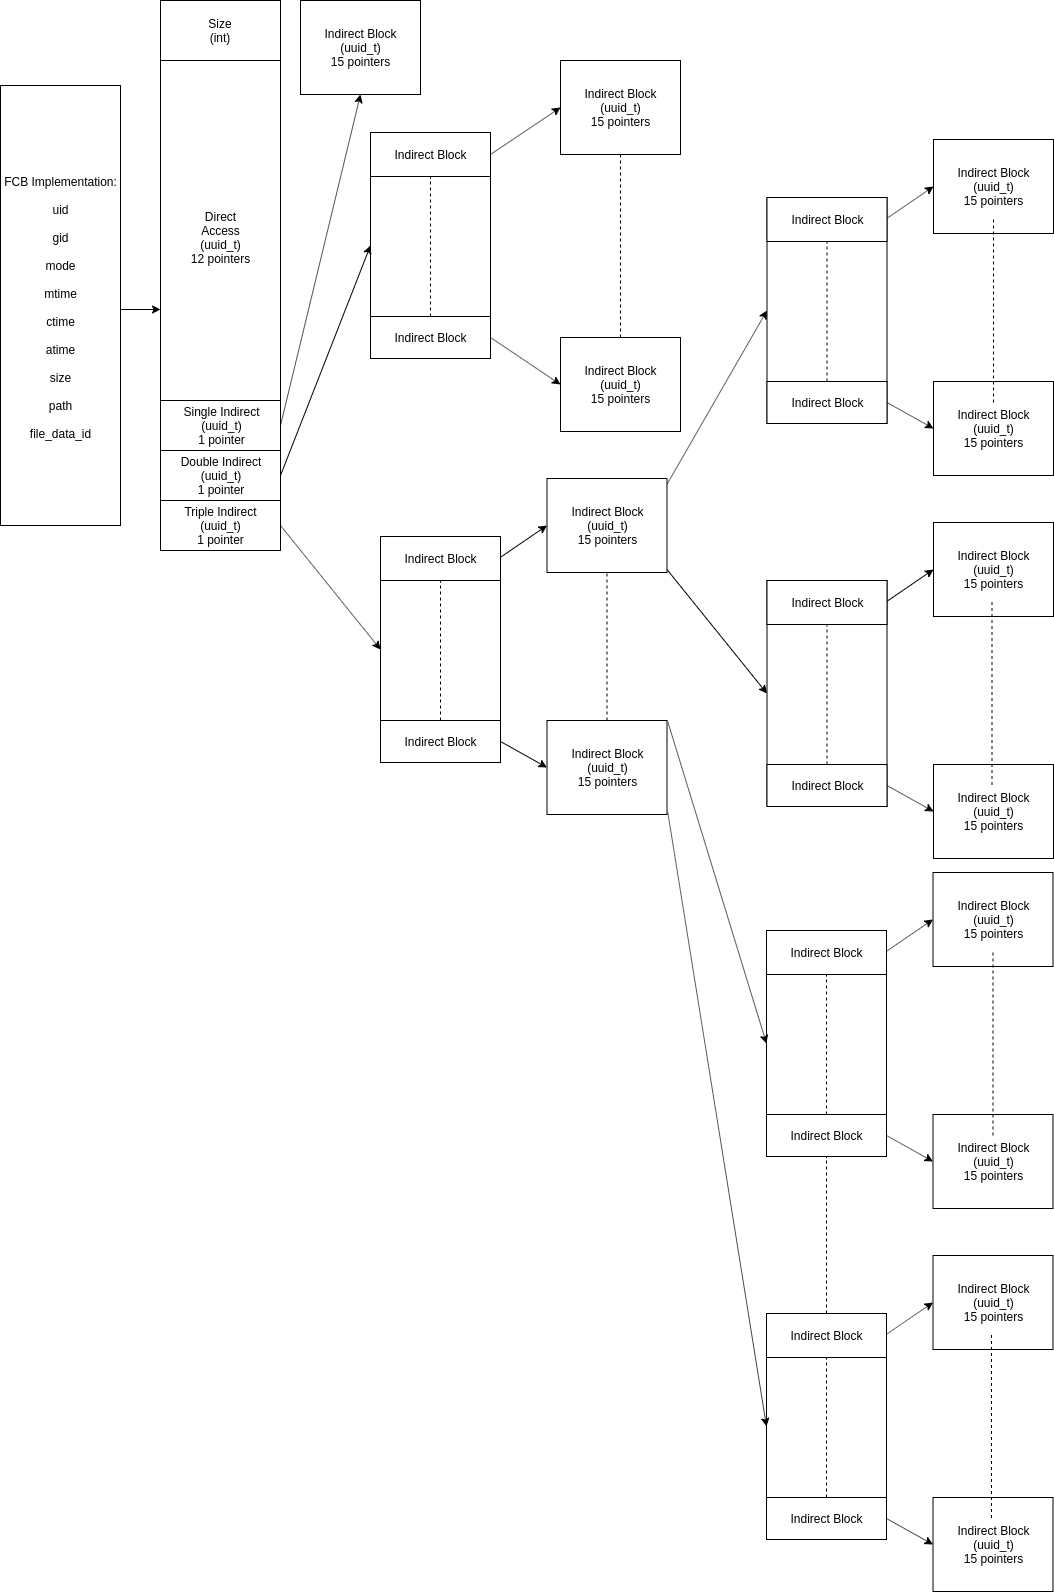
\includegraphics[width = \textwidth]{inode}
	\caption{Inode full design}
	\end{figure}
	There is a root inode in the memory with a simple and understandable key which can access the inode. For an arbitrary length file path and smaller memory use, we created a structure which mainly contains the key of the fcb and the name of the file.  This structure can be called entry, which is the entry of the fcb.\par
	For directories, entries will connect to the direct access pointer first. Only when the direct access pointer used up, it will generate an uuid and connect to the indirect pointers. Each indirect block has 15 pointers for connecting to different access blocks. So the single indirect entries will allows 15 entries, double indirect entries allows $15^{15}$ entries and triple indirect entries allows $15^{15^{15}}$ entries, which is actually big enough for storing all kinds of things.\par
	A improved design can be shows as follows:\par
	\begin{figure}[h!]
	\centering
	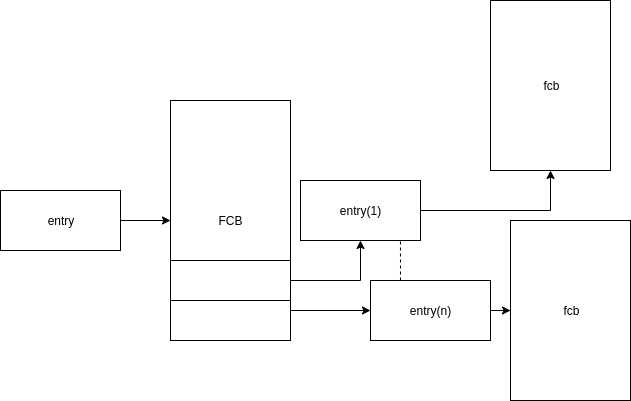
\includegraphics[width = \textwidth]{addnode}
	\caption{another design}
	\end{figure}
	FCB only pay response to other entries but does not care about fcbs. In a contract, entries only pay response to its FCB but does not pay attension on another entries. This makes finding specific file much easier, as each entry has a single path name and a single uuid key, which has an obvious advantage than the previous design.
	\section{Implementation}
	\subsection*{get attribute}
	This function will judge whether it is root file first, then if not it will directly access to the fcb of the path and retrieve the information of such block. 
	\subsection*{access to the path from local argument}
	This can be finished by using $strtok(str, "/")$
	\section{Testing}
	
	\section{Summary}
	This Practical is hard enough and time is not generally enough for finishing it. I am sad about I cannot finish the who implementation and leave a program with full of bugs. But I actually works for 40+ hours without any sleep, just my brain has stopped running and I am so tired to think anything. The only thing I can do is to finish the report and show my design and possible implementation. I am quite sorry about that.
\end{document}